\documentclass[11pt]{article}
\usepackage[utf8]{inputenc}

\usepackage{geometry}
\geometry{a4paper}

\usepackage{graphicx}
\graphicspath{ {./images/} }


\usepackage{amsmath}
\usepackage{booktabs} % for much better looking tables
\usepackage{array} % for better arrays (eg matrices) in maths
\usepackage{paralist} % very flexible & customisable lists (eg. enumerate/itemize, etc.)
\usepackage{verbatim} % adds environment for commenting out blocks of text & for better verbatim
\usepackage{subfig} % make it possible to include more than one captioned figure/table in a single float
% These packages are all incorporated in the memoir class to one degree or another...

\usepackage{fancyhdr} % This should be set AFTER setting up the page geometry
\pagestyle{fancy} % options: empty , plain , fancy
\renewcommand{\headrulewidth}{0pt} % customise the layout...
\lhead{}\chead{}\rhead{}
\lfoot{}\cfoot{\thepage}\rfoot{}

%%% SECTION TITLE APPEARANCE
\usepackage{sectsty}
\allsectionsfont{\sffamily\mdseries\upshape} % (See the fntguide.pdf for font help)
% (This matches ConTeXt defaults)

%%% ToC (table of contents) APPEARANCE
\usepackage[nottoc,notlof,notlot]{tocbibind} % Put the bibliography in the ToC
\usepackage[titles,subfigure]{tocloft} % Alter the style of the Table of Contents
\renewcommand{\cftsecfont}{\rmfamily\mdseries\upshape}
\renewcommand{\cftsecpagefont}{\rmfamily\mdseries\upshape} % No bold!

\usepackage[backend=bibtex,style=verbose-trad2]{biblatex}
\bibliography{bib} 

\title{EfficientDet-based Deep Learning Model for Detection and Classification of Malaria-Infected Human Blood Smears: An End-to-End Solution}
\author{Mohammad Mahdi Heydari}

\begin{document}
\maketitle

\section{Abstract}

Here we try to tackle the cell segmentation problem on the BBBC041\footnote{malaria infected human blood smears: https://bbbc.broadinstitute.org/BBBC041} dataset. The dataset's images contains 6 classes of cells in the blood stream and the goal is to find the cells coordinate and class for every cell which is present in the image. To accomplish this, a recently developed model named EfficientNet by google's brainAI team is utilized. By using this, the trained model succeeded to achieve map 52 over the test dataset.

\section{Dataset}

Images in this dataset contains 6 classes from two categories (infected and uninfected). for each image provided the annotation data which is bounding box coordinates and class for each cell. Although the author mentions that there exist only 6 classes, but a 7th class named "difficult" observed in the data which we ignored for training. Figure \ref{fig:class_freq} shows the class frequencies for each set.

\begin{figure}[!ht]
    \centering
    \caption{Class frequencies for dataset.}
        \subfloat[Train set class frequencies]{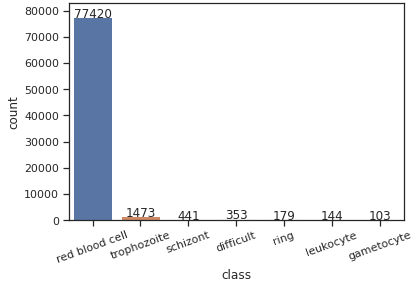
\includegraphics[width=0.4\columnwidth]{train-frequencies}}
        \qquad
        \subfloat[Test set class frequencies]{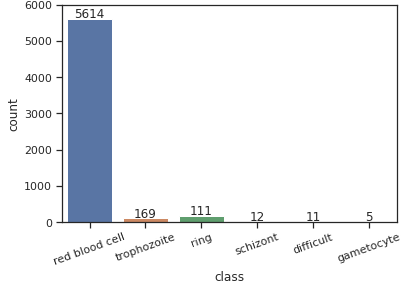
\includegraphics[width=0.4\columnwidth]{test-frequencies}}
    \label{fig:class_freq}
\end{figure}

To shrink the problem space, we added an extra preprocessing step and that would be removing the background using Otsu's method which is a automatic image thresholding technique. after downsclaing images to the network input size (512$\times$512 px) we perform otsu thresholding to find a binary mask over the cells. to make the mask smoother, we used morphological operations like binary\_closing and binary\_fill\_holes in order to keep entire cell area in image. for the final step, by dividing all pixel values to 255 the network input well always be a tensor sized 512$\times$512$\times$3 which it values is between 0 and 1 . Figure \ref{fig:pre} shoes the output of preprocessing step for some of training samples.

\begin{figure}[!ht]
	\centering
	\caption{Output of preprocessing step.}
	\subfloat{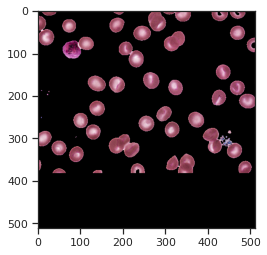
\includegraphics[width=0.29\columnwidth]{pre_1}}
	\qquad
	\subfloat{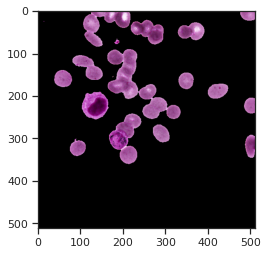
\includegraphics[width=0.29\columnwidth]{pre_2}}
	\qquad
	\subfloat{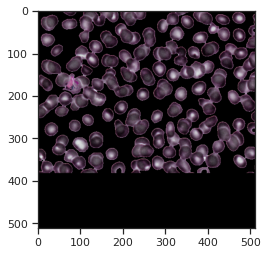
\includegraphics[width=0.29\columnwidth]{pre_3}}
	\label{fig:pre}
\end{figure}

\section{Related Works}

There are several Deep Leaning models for this task like Yolo, FasterRCNN and ... in this work we used a recently proposed model by Google brainAI team named EfficientDet. it's an scalable and efficient one-stage multi-scale object detector which achieved state-of-the-art results on Microsoft's COCO dataset.

\begin{figure}
	\centering
	\caption{Effect of increasing number of layers, channels and input resolution on model's accuracy}
	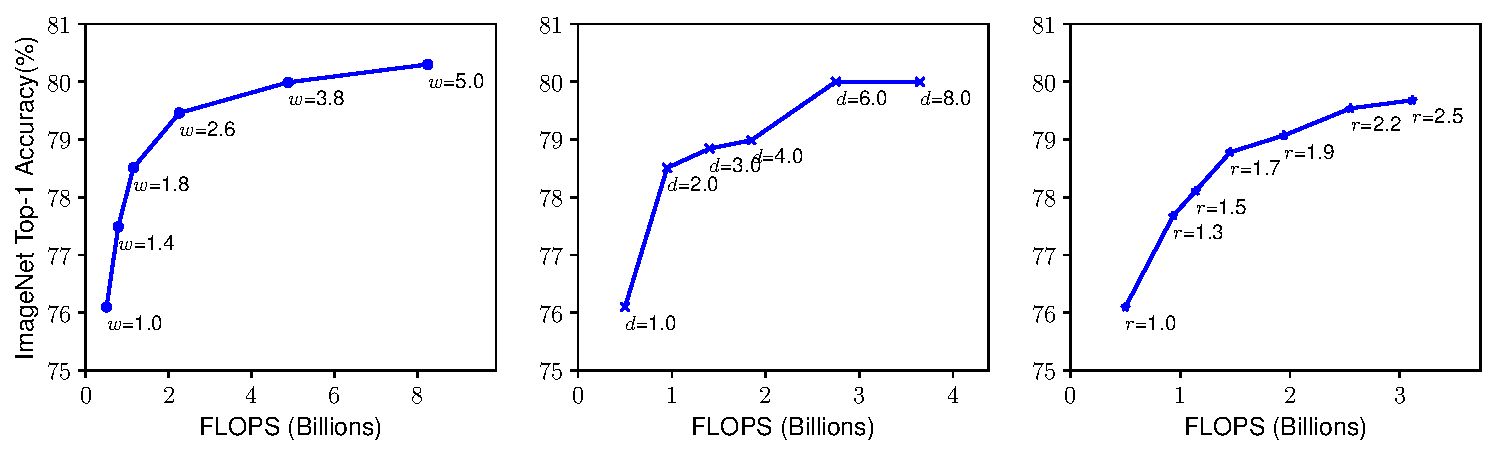
\includegraphics[width=1.0\textwidth]{scale-single}
	\label{fig:scale-single}
\end{figure}

EfficientDet is based on their previous work EfficientNet. the EfficientNet is a classifier model which built on famous MobileNet architecture. as the paper title suggests (Rethinking Model Scaling for Convolutional Neural Networks) they parameterized model's computational cost (flops) using number of layers, number of channels in each layer and input resolution of model. they showed that increasing number of layers or channels independently can increase the model accuracy to a point and after that accuracy will saturate (Figure \ref{fig:scale-single}). so they relate this three hyperparameter and optimized model's computational cost subject to them. they introduced  $\phi$ parameter as below:

\begin{equation}
	\label{eq:optobj} 
	\begin{aligned}
		\text{depth: } & d  = \alpha ^ \phi \\
		\text{width: } & w = \beta ^ \phi \\
		\text{resolution: } & r   =  \gamma ^ \phi  \\
		\text{s.t.    }  & \alpha \cdot \beta ^2 \cdot \gamma ^ 2 \approx 2 \\
		& \alpha \ge 1, \beta \ge 1, \gamma \ge 1 
	\end{aligned}
\end{equation}

so increasing $\phi$ will give us a more deeper and wider model which uses a higher resolution input. Result's on ImageNet dataset shows that it's actually quite effective in compare to the most recent methods (Figure \ref{fig:flops}).

\begin{figure}
	\centering
	\caption{Relation of $\phi$ with model's accuracy (B0 to B6)}
	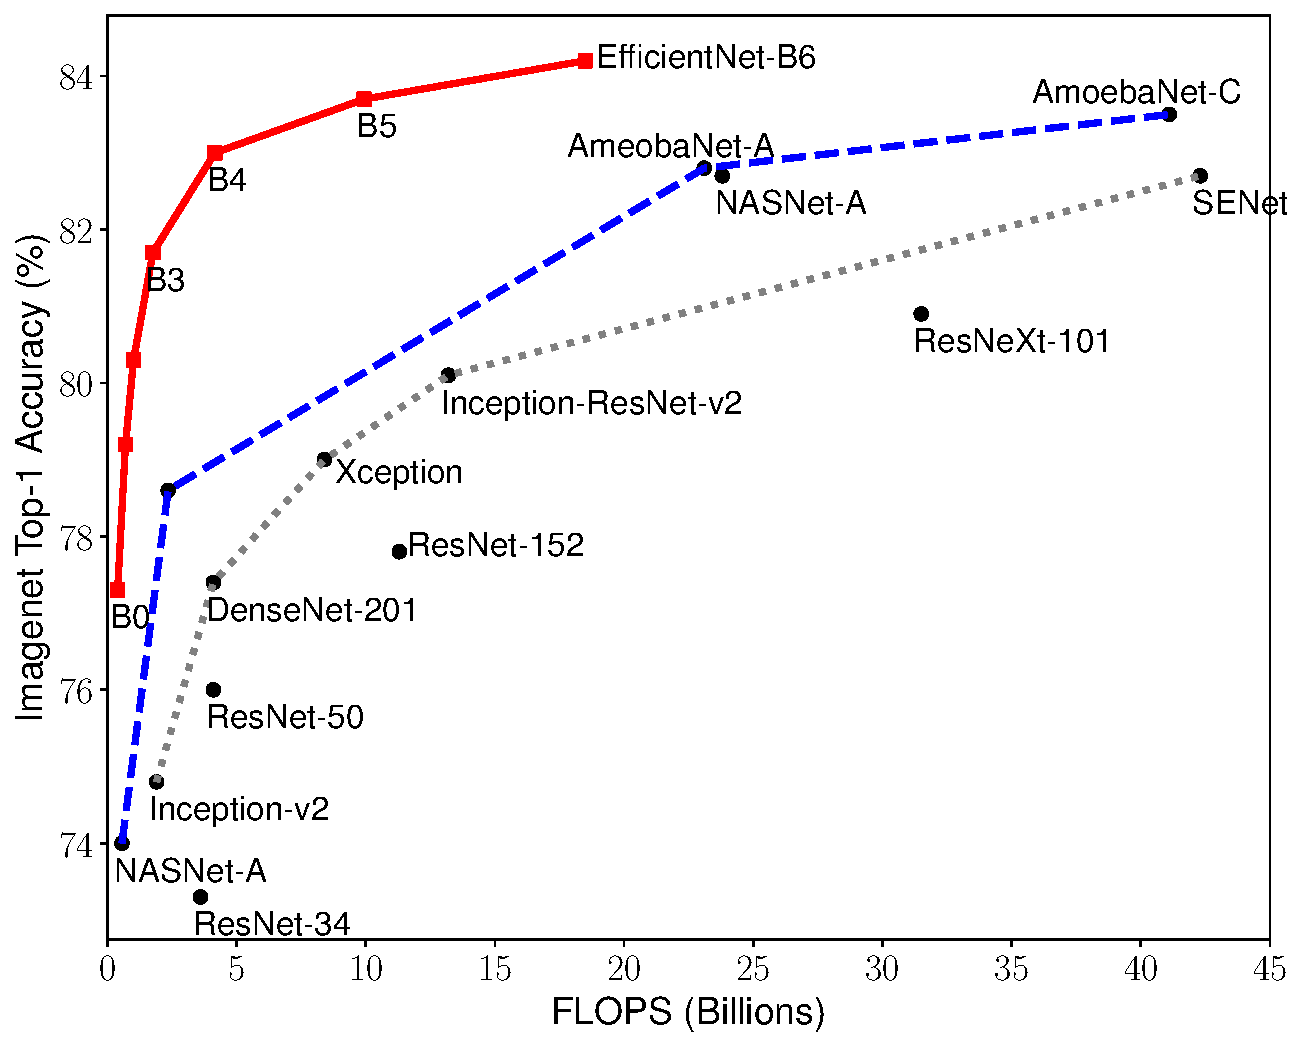
\includegraphics[width=0.7\textwidth]{flops}
	\label{fig:flops}
\end{figure}

\section{Poposed Model}

Following the EfficientDet architecture, we used EfficientNet $\phi = 0$ as backbone network which include multiple MBConvBlock layers to extract the feature map. Table \ref{tab:efficientnetb0} shows the overall properties of the blocks at the backbone network. we use level 3-7 level features from the backbone network and feed them into to BiFPN layers. this is where this multi-scale features fuse together with a top-down and bottom-up bidirectional feature fusion operation. then we feed them to box and class prediction networks to get the final result. Figure \ref{fig:efficientdetarch} shows the overall architecture of EfficientDet.

\begin{figure}
	\centering
	\caption{EfficientDet architecture}
	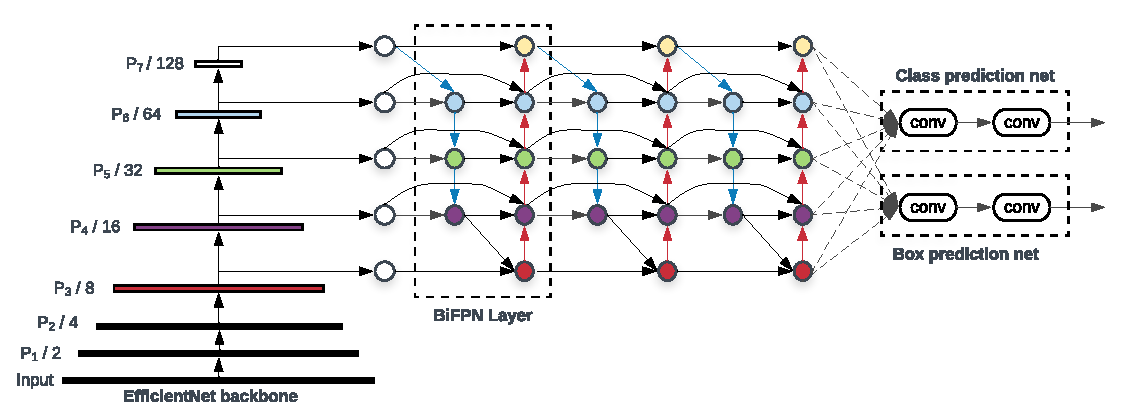
\includegraphics[width=1.0\textwidth]{efficientdetarch}
	\label{fig:efficientdetarch}
\end{figure}

\subsection{MBConvBlock}

MBConvBlock is the main building block of the backbone network which first introduced in MobileNet V2. each block contains this phases (copied from the paper):

\begin{itemize}
	\item{\textbf{Expansion phase:} we will expand our layer and make them wide as mentioned in Inverted residual block (connected blocks are narrow and inner blocks are wider, here we are making layer wider just by increasing the number of channels).}
	
	\item{\textbf{Depthwise convolution phase:} after expansion, we perform depthwise convolution with kernel size mentioned in block argument.}
	
	\item{\textbf{Squeeze and excitation phase:} now, we extract global features with global average pooling and squeeze numbers of channels. the output of this phase can be considered as weightage for each channel in the output.}
	
	\item{\textbf{Output phase:} after the squeeze and excitation, we apply convolution operation that gives output filters mention in the argument block.}
\end{itemize}

\subsection{Swish Activation}

to resolve the ReLu's problem with negative values brainAi team introduced a new activation function named Swish:

\begin{equation}
	\label{eq:swish}
	\text{$Swish(x) = x * sigmoid(x)$}
\end{equation}

they proved using swish activation function the $InceptionResNetV2$ achieve 0.6\% more accuracy on the ImageNet dataset.

\subsection{BiFPN network}

this layer doing bidirectional cross-scale connections
and weighted feature fusion and originally introduced in the efficientDet's paper. given a list of multi-scale features $\vec{P}^{in} = (P^{in}_{l_1}, P^{in}_{l_2}, ...)$, the goal is to find a transformation $f$ that can effectively aggregate different features and output a list of new features: $\vec{P}^{out} = f(\vec{P}^{in})$. in this work we implemented \textit{Fast normalized fusion} which introduced in the paper. $O = \sum_{i} \cfrac{w_i}{\epsilon + \sum_{j} w_j} \cdot I_i$, where $w_i \ge 0$ is ensured by applying a Relu after each $w_i$, and $\epsilon = 0.0001$ is a  small value to avoid numerical instability. for example here we describe the two fused features at level 6 for BiFPN:

\begin{align*} 
	P^{td}_6 &= Conv\left(\frac{w_1\cdot P^{in}_6  +     w_2 \cdot Resize(P^{in}_7)}{w_1 + w_2 + \epsilon}\right) \\
	P^{out}_6 &= Conv\left(\frac{w'_1\cdot P^{in}_6  +  w'_2 \cdot P^{td}_6 + w'_3 \cdot Resize(P^{out}_5)}{w'_1 + w'_2 + w'_3 + \epsilon}\right)
\end{align*}

where $P^{td}_6$ is the intermediate feature at level 6 on the top-down pathway, and $P^{out}_6$ is the output feature at level 6 on the bottom-up pathway. All other features are constructed in a similar manner. (this part is copied from the original paper)

\begin{table}
	% \vskip -0.1in     
	\caption{Backbone layers}
	% \vskip 0.05in
	\centering   
	
	\resizebox{1.0\columnwidth}{!}{ 
		\begin{tabular}{c|c|c|c|c|c}                
			\toprule[0.15em]                                                                  
			Stage & Operator  & Resolution      & \#Channels & stride & \#Layers \\
			$i$ &   $\mathcal{ \hat F}_i$ & $ \hat H_i \times  \hat W_i $     &  $ \hat  C_i$ & & $ \hat L_i$        \\
			\midrule                                                              
			- &    Conv3x3       & $ 256 \times 256 $   & 32 & 2 & 1 \\
			
			
			
			
			- &   MBConv1, k3x3  & $ 256 \times 256 $   & 16 & 1 & 1 \\
			
			
			
			
			
			- &   MBConv6, k3x3  & $ 128 \times 128 $   & 24 & 2 & 2 \\
			
			
			
			
			
			
			
			P\subfloat{3} &   MBConv6, k5x5  & $  64 \times 64  $   & 40 & 2 & 2  \\
			
			
			
			
			
			
			- &   MBConv6, k3x3  & $  32 \times 32  $   & 80 & 2 & 3 \\
			
			
			
			
			
			P\subfloat{4} &   MBConv6, k5x5  & $  32 \times 32  $   & 112 & 1  & 3 \\
			
			
			
			- &   MBConv6, k5x5  & $  16 \times 16  $   & 192  & 2 & 4  \\
			
			
			P\subfloat{5} &   MBConv6, k3x3  & $   16 \times 16   $   & 320 & 1 & 1  \\
			
			- &    Conv3x3       & $ 16 \times 16 $   & 64 & 2 & 1 \\
			P\subfloat{6} &    MaxPool3x3       & $ 8 \times 8 $   & 64 & 2 & 1 \\
			P\subfloat{7} &    MaxPool3x3       & $ 4 \times 4 $   & 64 & 2 & 1 \\
			\bottomrule[0.15em]                                                                     
		\end{tabular}                                                                  
	}                                                                                 
	
	\label{tab:efficientnetb0}      
\end{table} 

\subsection{Focal Loss}

duo to huge the amount of pixel belongs to the background in compare of pixels which belongs to the actual objects, there is a large imbalance between class frequencies. to solve that we used Focal Loss with below formula to assign bigger penalty to the model for misclassifying the object's pixels:

\begin{equation}
	\label{eq:focal}
	\text{$ FL(P_{t}) = - (1 - P_{t})^{\gamma} Log(P_{t}) $}
\end{equation}

\section{Results}

we trained the model with 100 epochs with Adam optimizer (10\textsuperscript{-4} learning rate) which took near 3 hours on the 80\% random part of the train set and used the other 20\% as validation data. Figure \ref{fig:loss_2} shows the loss of the model for train and validation set during the training process. Figure \ref{fig:out} shows the final results on some of the test images. we clearly can see the model does a perfect job in locating the cells, the classification results are so bad that isn't worth mentioning.

\begin{figure}
	\centering
	\caption{Model's loss along training}
	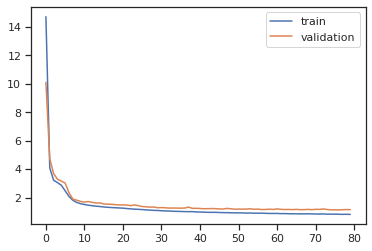
\includegraphics[width=0.6\textwidth]{loss_3}
	\label{fig:loss_2}
\end{figure}

\begin{figure}[!ht]
	\centering
	\caption{Output of trained model on the test set.}
	\subfloat{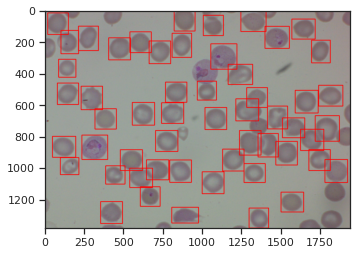
\includegraphics[width=0.29\columnwidth]{out_1}}
	\qquad
	\subfloat{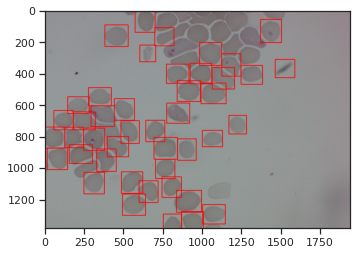
\includegraphics[width=0.29\columnwidth]{out_2}}
	\qquad
	\subfloat{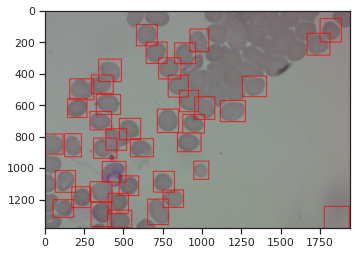
\includegraphics[width=0.29\columnwidth]{out_3}}
	\label{fig:out}
\end{figure}

\section{Discussion}

Speaking around the poor performance of the model, it did a perfect job in predicting bounding boxes but the classification result is worthless, the output is "red blood cell" for every thing. one reason for this is a huge class imbalance which in this context can't be solve with data augmentation or bootstrapping. one way to solve this issue is using the $\alpha$ parameter in the focual loss, although we tried playing around this but didn't help much in the first shot and need more work to solve the issue.

Using one-stage detectors are fairly rare in this context which i believe mostly is because the common pattern in cell shapes makes it easy for two-stage detectors. Although the EfficientDet architecture is the state-of-the-art result holder for 90-class COCO dataset, it did poor job solving this problem. it's good to mention that the thresholding method helped model by a lot but it is not a common and standard procedure using this kind of models. this model is designed to be an end-to-end solution.

Our intent in using this architecture was try to implement a new state-of-the-art model and after spending a lot of time it was unpleasant to ignore it.

\nocite{*}

\printbibliography[title={Reference}]

\end{document}
